\section{EAC}
\label{sec:eac results}

This section will present thorough results concerning several characteristics related to the EAC method.
These were the timings of the different parts, how cardinality and the different $K_{min}$ rules affected the sparsity of the co-association matrix, the typical number of associations per cluster in each rule, the growth of the number of associations with the different parameters, among others.
Two mixture of Gaussians of 6 clusters, 10 million patterns and two dimensions were generated.
A variation of the number of dimensions has more interest in the production phase.
Since the production of the ensemble uses K-Means, detailed results can be found in section \ref{sec:parallel kmeans}.
One mixture has overlapping Gaussians and the other does not.
The reasoning was that overlapping Gaussians might result in more associations per cluster.

Throughout this section, different rules for computing the $K_{min}$ and different co-association matrix formats will be mentioned.
The different formats for the co-association matrix have been presented in chapter \ref{chapter:methodology}.
The different rules and their aliases are presented in Table \ref{tab:eac rules}.

\begin{table}[h]
\centering
\caption{Different rules for computing $K_{min}$ and $K_{max}$. $n$ is the number of patterns in the data set and $sk$ is the number of samples per cluster.}

\begin{tabular}{lcc}
\toprule
Rule &  $K_{min}$ &  $K_{max}$ \\
\midrule
\emph{sqrt}     & $\frac{\sqrt{n}}{2}$      & $\sqrt{n}$    \\
\emph{2sqrt}    & $\sqrt{n}$                & $2 \sqrt{n}$  \\
\emph{sk=sqrt2} & $sk = \frac{\sqrt{n}}{2}$ & $1.3 K_{min}$ \\
\emph{sk=300}   & $sk = 300$                & $1.3 K_{min}$ \\
\bottomrule
\end{tabular}

\label{tab:eac rules}
\end{table}

The experiment that generated the results of these section was set up as follows.
A large data set was generated.
The data set was sampled uniformly to produce a smaller data set with the desired number of patterns.
A clustering ensemble was produced (production phase) for each of these smaller data sets and for each of the rules, using K-Means.
From each ensemble, co-association matrices of every applicable format were built (combination phase).
A matrix format was not applicable when the data set complexity would make its correspondent co-association matrix too big to fit in main memory.
The final clustering (recovery phase) was also done for each of the matrix formats.
SLINK was used with fully allocated formats and the MST-based SL (SL-MST) and MST-based SL on external memory (SL-MST-disk) were executed with sparse matrices.
SL-MST was not executed if its space complexity was too big to fit in main memory.
Furthermore, the combination and recovery phases were repeated several times for smaller data sets for statistical relevant of the execution times, so as to make the influence of any background process less salient.
For big data sets, the execution times are big enough that the influence of background processes is negligible.

\subsubsection{Building the co-association matrix}

The execution times for building the co-association matrix can be observed in Figures \ref{fig:eac build rules
} and \ref{fig:eac build matrices}.
The different 
It is clear from Fig. \ref{fig:eac build rules} that as 

\begin{figure}[hbtp]
    \centering
    \includegraphics[width=0.8\textwidth]{{{results/eac/build_time/sparse_condensed_linear}}}
    \caption{Execution time for building the co-association matrix from ensemble with different rules.}
    \label{fig:eac build rules}
\end{figure}

\begin{figure}[hbtp]
    \centering
    \includegraphics[width=0.8\textwidth]{{{results/eac/build_time/2sqrt}}}
    \caption{Execution time for building the co-association matrix with different matrix formats.}
    \label{fig:eac build matrices}
\end{figure}

\subsubsection{SLINK vs SL-MST vs SL-MST-Disk}

The clustering times don't change significantly for the different rules.

\begin{figure}[hbtp]
    \centering
    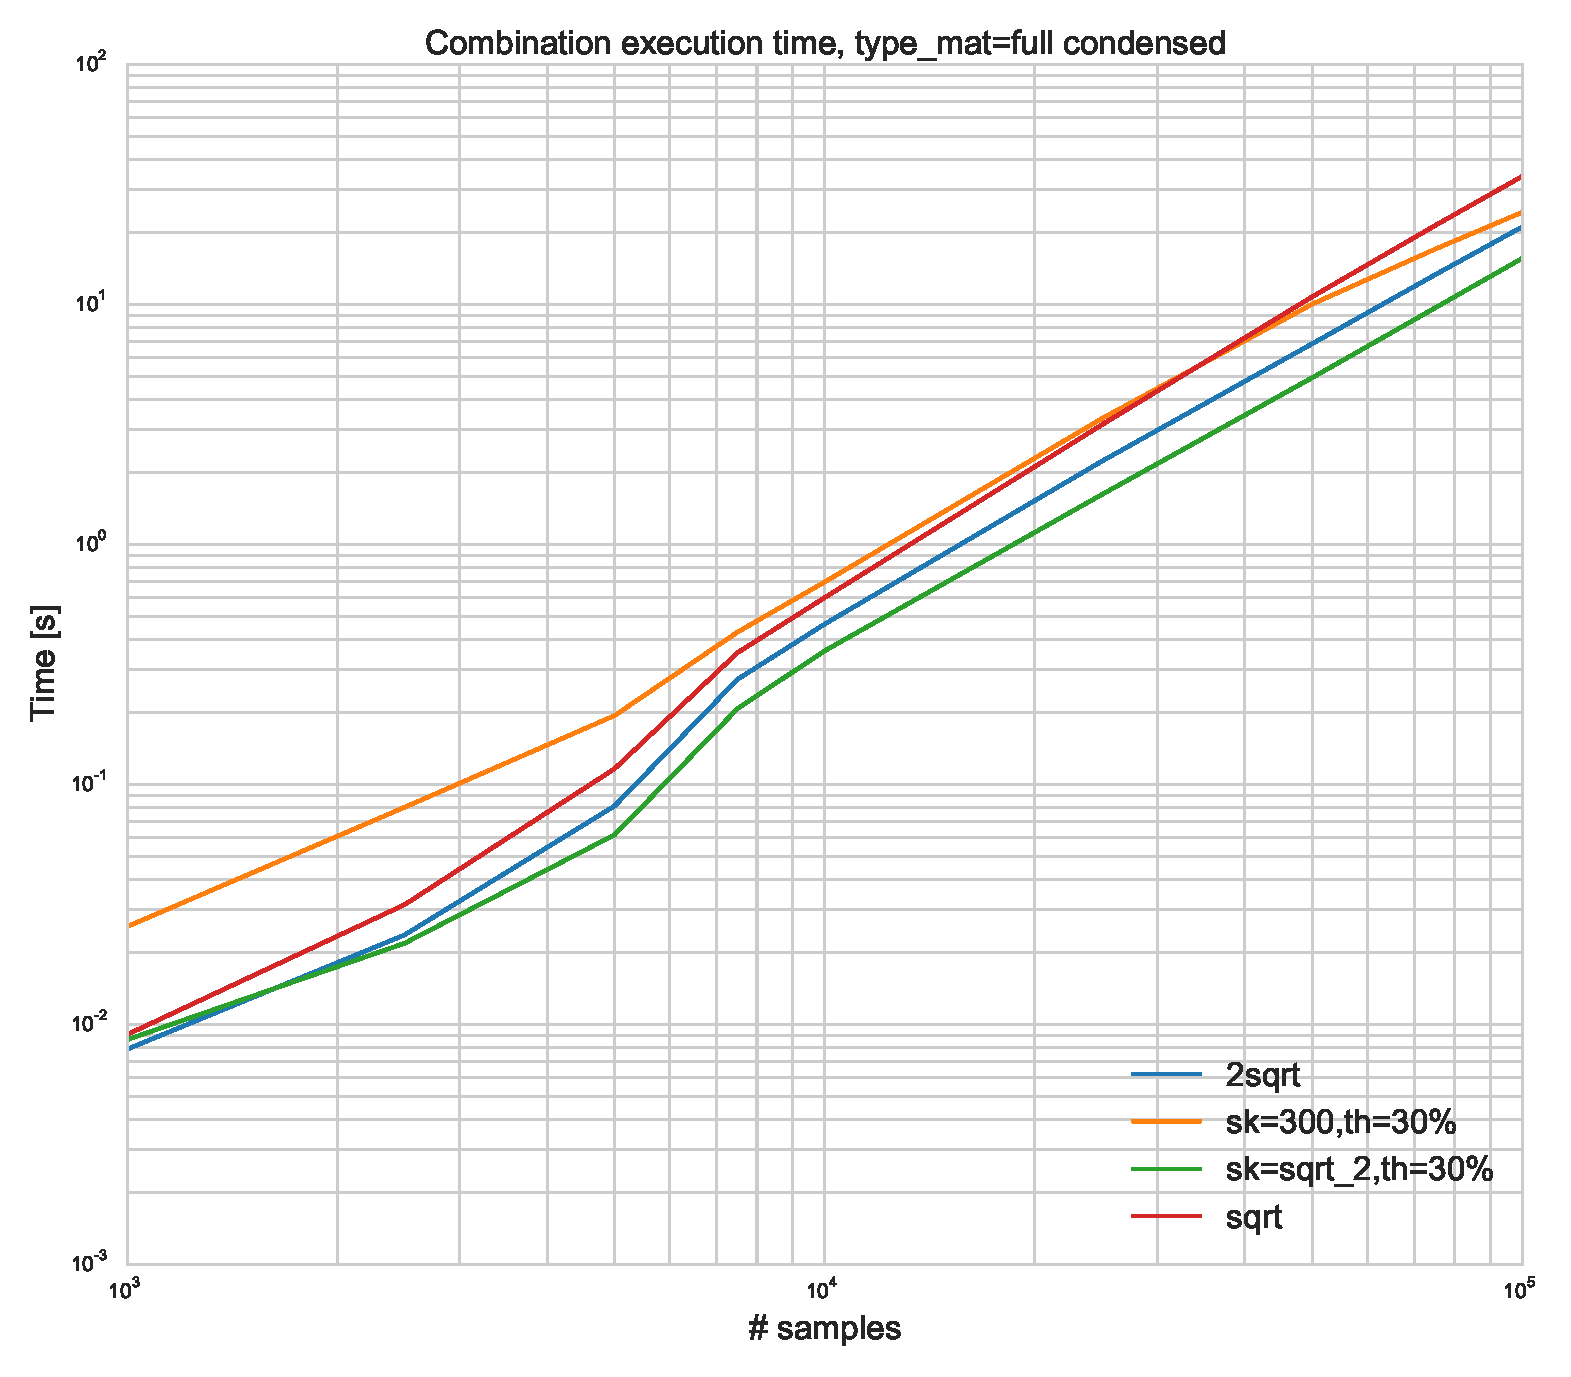
\includegraphics[width=0.8\textwidth]{{{results/eac/sl_mem_time/full_condensed}}}
    \caption{Comparison between the execution times of SLINK to different rules.}
    \label{fig:sl full condensed}
\end{figure}

\begin{figure}[hbtp]
    \centering
    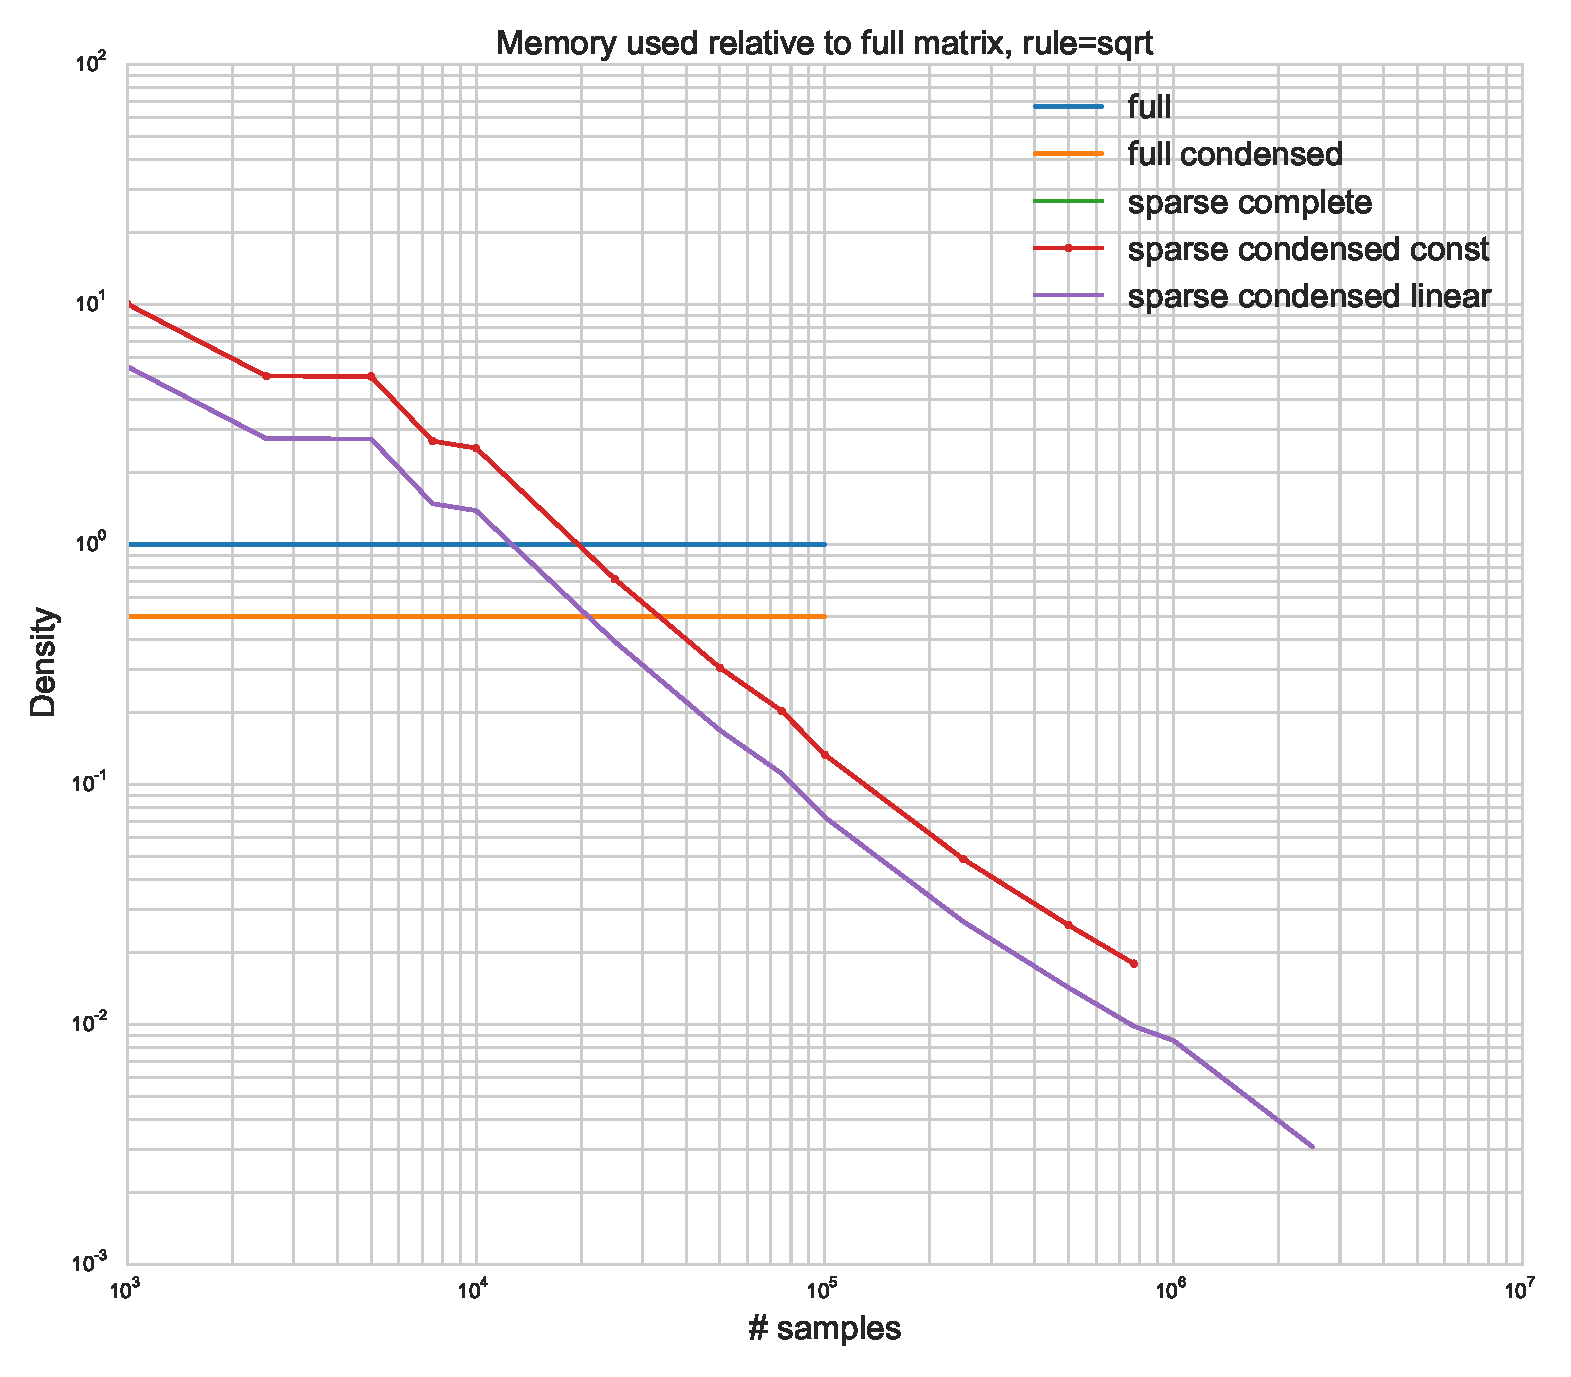
\includegraphics[width=0.8\textwidth]{{{results/eac/sl_time/sk=300}}}
    \caption{Comparison between the execution times of the three methods of SL over condensed matrices. SLINK runs over fully allocated condensed matrix while SL-MST and SL-MST-Disk run over the sparse matrix.}
    \label{fig:sl time}
\end{figure}

\subsection{Number of associations, allocated associations and actual used memory}

The sparse nature of EAC has been referred to before and that is clear in Fig. \ref{fig:eac assoc density}.
This figure shows the actual density of associations that the co-association matrix for the different data sets and rules relative to the $n^2$ space of the full matrix.



\begin{figure}[hbtp]
    \centering
    \includegraphics[width=0.8\textwidth]{{{results/eac/assoc_density/sparse_condensed_linear}}}
    \caption{Density of associations relative to the full co-association matrix, which hold $n^2$ associations.}
    \label{fig:eac assoc density}
\end{figure}

\begin{figure}[hbtp]
    \centering
    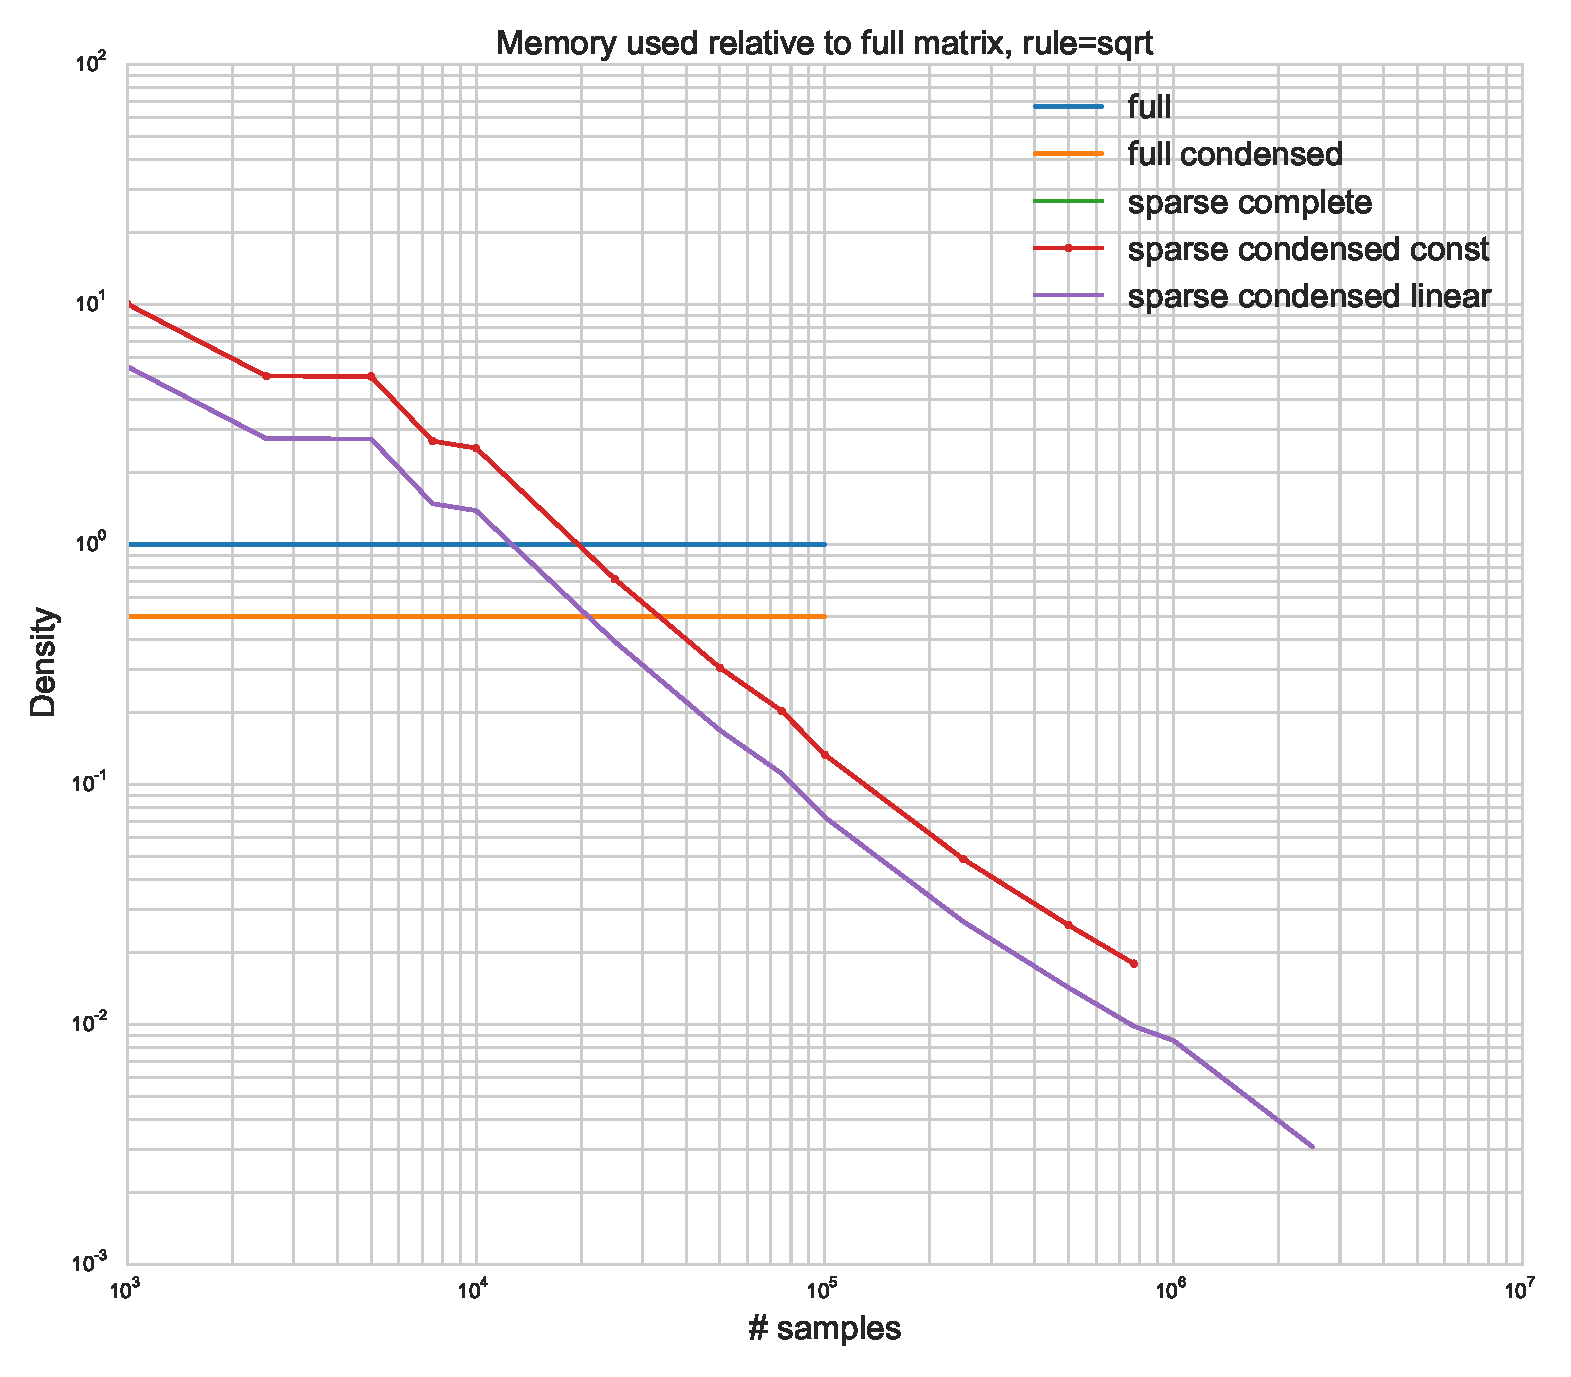
\includegraphics[width=0.8\textwidth]{{{results/eac/sl_time/sk=300}}}
    \caption{Comparison between the execution times of the three methods of SL over condensed matrices. SLINK runs over fully allocated condensed matrix while SL-MST and SL-MST-Disk run over the sparse matrix.}
    \label{fig:sl time}
\end{figure}


